\documentclass[../../report.tex]{subfiles}
\begin{document}
\section{Spiking Neural Networks}

Nowadays, the most successful ANN sequence modelling techniques contain on the
order of hundreds of millions of parameters \cite{Bender2021}. Such scale endows
these models with impressive capabilities. For instance, Google's BERT achieved
state-of-the-art performance on natural language understanding benchmarks
\cite{Devlin2019}. However, training BERT consumes 12 kilowatts of power
\cite{Strubell2019}. Meanwhile, human brains seem to have no problem processing
language with a measly few tens of watts. Although such a comparison is a gross
oversimplification, it nevertheless highlights a major discrepancy between
artificial and biological intelligence.

Biologically inspired spiking neural networks (SNNs) aim to demystify the
efficiency of the brain. And with the advent of neuromorphic computing platforms
such as SpiNNaker \cite{Furber2014} and Intel Loihi \cite{Davies2018},
simulating brain-like circuits is becoming feasible.

\subsection{Neuron model}

For the purposes of this project, neurons shall be implemented according to the
prominent \emph{leaky integrate-and-fire} (LIF) model. LIF neurons are shapeless
entities that accumulate incoming weighted \emph{spikes} in the form of a
\emph{membrane potential}. If this potential exceeds a threshold, the neuron
emits a unitary spike itself, and the potential resets (figure
\ref{fig:neuron}). Otherwise, the membrane potential decays over time back to a
resting level. Moreover, following a spike, the neuron enters a short
\emph{refractory period}, during which it cannot spike again, regardless of
incoming stimulus.

\begin{figure}
  \centering
  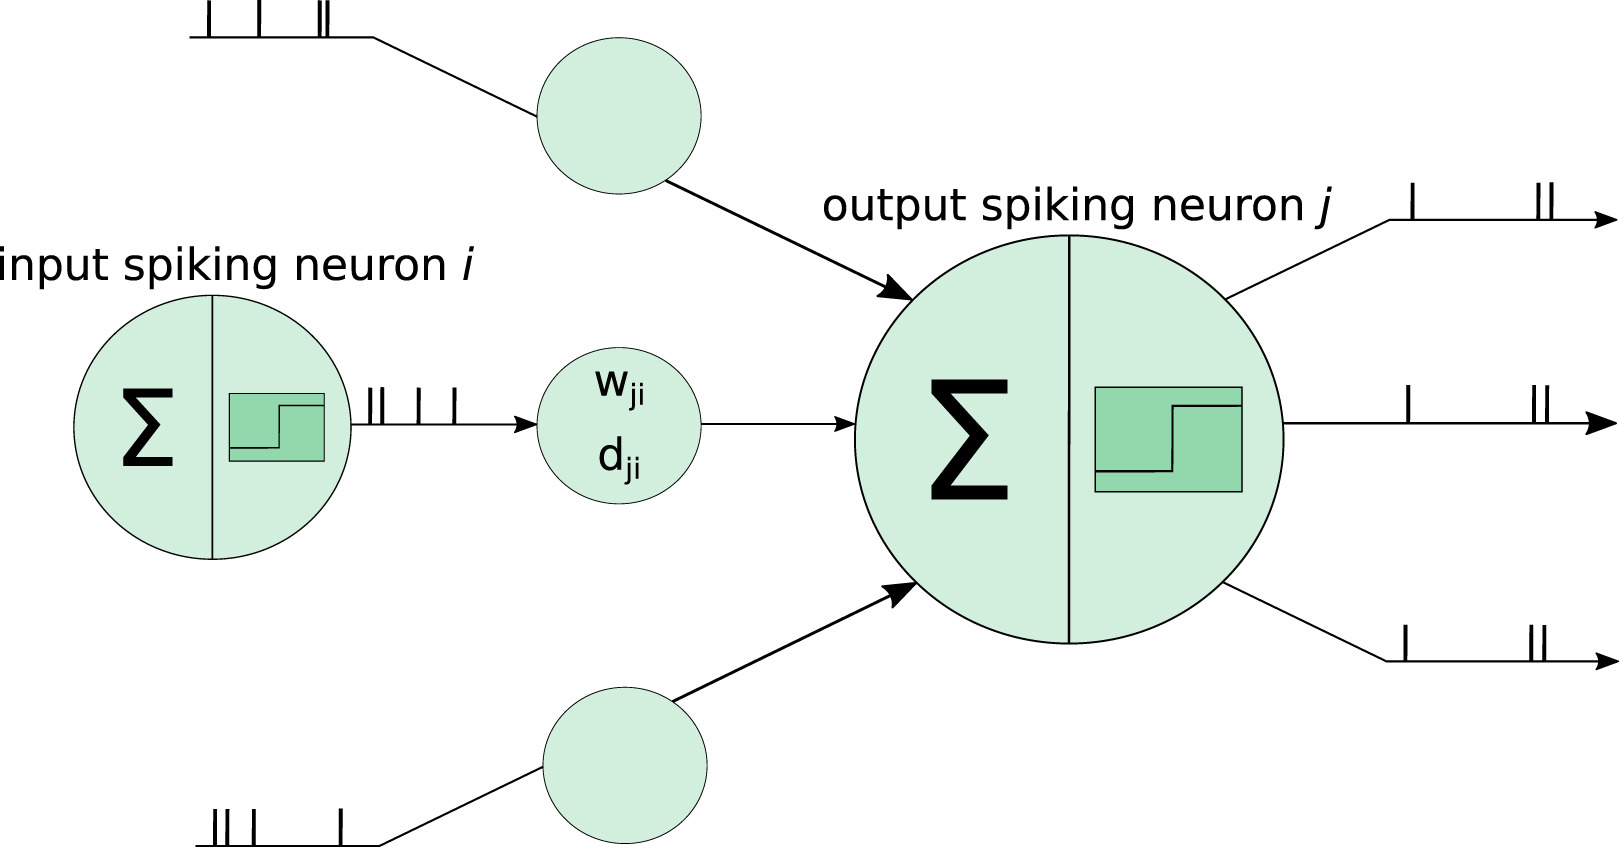
\includegraphics[width=0.75\textwidth]{neuron}
  \caption{Computational model of a neuron \cite{Lobo2020}}
  \label{fig:neuron}
\end{figure}

\subsubsection{Neuronal adaptation}
The standard LIF model omits an important property observed in experimental
evidence -- spike frequency adaptation. When stimulated with a constant input
current, many neurons exhibit a reduction in firing rate after the initial burst
of spikes. This means that effectively, their firing threshold increases. It has
been shown that an SNN with such adaptive LIF (ALIF) neurons gains memory
capabilities similar to that of an LSTM \cite{Bellec2018LSNN}, and therefore
such a configuration is known by the portmanteau LSNN.

\subsection{Plasticity}

The brain's learning mechanism is not well understood beyond the scale of
individual synapses. Experimental evidence has shown that the strength of
synaptic connections is modified based on the relative spike timings of the pre-
and post-synaptic neurons \cite{Bliss1973}. This learning rule is known as
spike-timing-dependent plasticity (STDP). Unfortunately, it is intrinsically a
form of unsupervised learning, making it unsuitable for our task of melody
generation.

It is unclear how the brain coordinates these synaptic updates to achieve
specific goals. Although there is hope that this process may share conceptual
similarities with backpropagation \cite{Lillicrap2020}, it is unlikely that the
brain employs backpropagation \emph{through time}, primarily because BPTT
requires storing past neuron states for error signal computation
\cite{Lillicrap2019}. Nevertheless, it is possible to train SNNs with BPTT, as
long as the discontinuous spike function is replaced by a differentiable
alternative \cite{Bellec2018LSNN}.

\subsection{Biological plausibility}

Traditional ANNs have the freedom to diverge from biological realism, and to do
whatever gives good results. SNNs have not yet outperformed ANNs, but it is
clear that human brains are still superior at many tasks. This seems to suggest
that going forward, there is much to be learned from biology.

Indeed, a recently published SNN training algorithm, \emph{e-prop}, draws
inspiration from experimental neuroscience. Instead of propagating gradients
back in time like BPTT, e-prop accumulates local traces of potentially
correlated firing activity into the future. These traces are later combined with
network error signals\footnotemark{} to perform synaptic updates.
\cite{Bellec2020}

\footnotetext{In this sense, the role of the loss function becomes similar to
that of biological top-down signals, such as dopamine.}

Moreover, it is possible to augment the loss function with penalties that
encourage the network to exhibit biologically realistic behaviour. For example,
the inclusion of an averaged firing frequency target term prevents physically
impossible spike rates \cite{Bellec2018LSNN}.

\end{document}
